\documentclass[conference]{IEEEtran}
\usepackage[T1]{fontenc}
\usepackage{graphicx}
\usepackage{booktabs}
\usepackage{array}
\newcolumntype{L}[1]{>{\raggedright\arraybackslash}p{#1}}
\usepackage{amssymb}
\usepackage{stfloats}
\usepackage{microtype}
\usepackage{url}
\usepackage[hidelinks]{hyperref}

\newcommand{\K}{$K$}
\newcommand{\x}{$\times$}
\newcommand{\pick}{$^\star$}
\newcommand{\pickf}{$^{\star-}$}
\newcommand{\topk}{$^\dagger$}
\newcommand{\calc}{$^\ddagger$}
\newcommand{\late}{$^\S$}
\newcommand{\cfg}[1]{\texttt{#1}}
\setlength{\textfloatsep}{9pt plus 2pt minus 2pt}
\setlength{\dbltextfloatsep}{9pt plus 2pt minus 2pt}

\begin{document}

\title{Memory-Aware Agent Edge Serving\\
\large Phase 2: Agent-Level KV Lifecycle at Tool-Call Boundaries}

\author{\IEEEauthorblockN{Jiawei Liu, Kaiqi Han, Tianyu Xu, You Chen, Yufan Shi}
\IEEEauthorblockA{CSE 291A, Fall 2026}}

\maketitle

\section{Mechanism}

Phase~1 showed that under a tight KV budget a fixed concurrency \K{} must cover all \K{} agents'
simultaneous peaks: contexts grow 2--4\x{} per task and over-committing the pool fails every
in-flight request, while agents in tool calls hold 36--44\% of the KV. Phase~2 adds a client-side
KV manager that uses only \texttt{llama-server}'s~\cite{llamacpp} HTTP controls (\texttt{/completion}
with \texttt{id\_slot}, slot save/restore/erase, \texttt{/tokenize},
\texttt{/slots}); llama.cpp and the agent are unchanged.

\emph{(1) Ledger and gate.} Each slot is charged its exact resident count
$s_k=\mathit{prompt\_n}+\mathit{cache\_n}+\mathit{predicted\_n}-1$, or $\max(s_k,f)$ while a request
with $f=\mathrm{tok}(P)+n_\mathrm{predict}$ runs. A request dispatches only if
$U-u_k+\max(s_k,f)\le c-m$ ($U$: total charge, $c$: pool, $m=128$). If \texttt{/tokenize} is exact
(it matched the server on 550/550 prompts) and charges fall only after responses, this excludes
overflows and server purges. None occurred in 53 full-gate runs, which also had no ledger
violations or failed restores, and $\max U\le c-m$.
\emph{(2) Admission.} A task is admitted while all agents' projected peaks (size plus the
0.9-quantile of remaining growth, fitted on Phase~1 runs) fit $(1+\omega)(c-m)$, up to
$K_\mathrm{max}=8$ (delay \x1) or 16 (\x4).
\emph{(3) Lifecycle.} On a gate deficit, idle agents are
evicted one at a time, the one expected to return last first; an online cost model picks
\emph{offload} to host RAM ($h\cdot c$ tokens, $h=1$), \emph{drop} to the shared 1,421- or
1,633-token ReAct prefix, or \emph{erase}. Returning agents reclaim memory at once; new tasks take
idle KV only after a pressure-gated ski-rental TTL. Nothing is evicted without pressure
(see Table~\ref{tab:runtime}).


\section{Setup}

Runtime and workload are Phase~1's: \texttt{llama-server} b11960 on an A10G, Qwen2.5-7B-Instruct
Q4\_K\_M~\cite{qwen} with f16 KV in one unified pool, and HotpotQA ReAct agents~\cite{hotpotqa,react}
in the long-context mix (70\% \texttt{react\_long}): 200 tasks released at $t=0$, lognormal tool
delays (median 0.8\,s) scaled by \x1 or \x4. A point such as 16k\,\x4 names pool $c$ and delay
scale. B1 is Phase~1's FIFO fixed \K{} with pinned slots; B2 is llama.cpp's host cache (\texttt{-{}-cache-ram} $h\cdot c$,
\texttt{-{}-cache-idle-slots}, unpinned) with ours' host RAM on dev; B3 (per-slot regions) lost
20--29\% in tuning and was dropped; \cfg{ours\_h0} has no host tier. Knobs (\K, $\omega$) are tuned
on the perf split, one run each: the best goodput among knobs completing ${\ge}95\%$ (\pick;
\pickf: none does), plus B1's best-goodput \K{} (\topk). Evaluation uses fresh dev-split runs
(3 reps at 16k\,\x4 and 32k\,\x4, 2 at 8k\,\x1 and 16k\,\x1); 16k\,\x4 and 8k\,\x1 are the
headline points, 16k\,\x1 and 32k\,\x4 pre-registered low-benefit points. Goodput is EM-correct
tasks/min over the whole run, failures counted wrong. A difference is \emph{supported} (S) only if
Welch's $p<0.05$ on per-run goodput \emph{and} the bootstrap 95\% CI of the steady-window
difference excludes 0, else \emph{not established} (n.e.); quality uses paired per-question F1
TOST ($\pm0.05$).

\begin{table}[t]
  \caption{Runtime Facts Behind the Design (b11960, A10G)}
  \label{tab:runtime}
  \centering
  \scriptsize
  \setlength{\tabcolsep}{2.5pt}
  \begin{tabular}{@{}L{0.13\columnwidth}L{0.55\columnwidth}L{0.28\columnwidth}@{}}
    \toprule
    Probe & Observation & Consequence \\
    \midrule
    Idle slots & 4 decoders: 293 $\rightarrow$ 203 tok/s with 16 idle \x{} 3k; attention spans up
      to the top occupied cell & eviction saves compute only if it frees top cells \\
    Drop to prefix & prefix ids with $n_\mathrm{predict}=0$: 19.6\,ms; revisit reuses all 1,421 &
      keep the prefix \\
    Busy slot & save is deferred until the stream ends & ops on idle slots only \\
    Save, restore & 59.0 + 30.0\,\textmu s/tok in the probe (fragmented; online fit under load:
      83--245) vs.\ 281\,\textmu s/tok re-prefill & offload can beat re-prefill for long tails \\
    Pool full & idle slots purged in id order, then all processing slots fail & active KV is a
      hard limit \\
    Host cache & \texttt{-{}-cache-ram} saves and clears idle slots at each launch; pinned slots
      never reload & B2 runs unpinned \\
    \bottomrule
  \end{tabular}
\end{table}

\begin{table*}[!t]
  \caption{Main Comparison on the Dev Split (200 Tasks per Run; Mean over Reps, Min--Max)}
  \label{tab:main}
  \centering
  \scriptsize
  \setlength{\tabcolsep}{3.2pt}
  \renewcommand{\arraystretch}{0.9}
  \begin{tabular}{@{}lllrcrcrrrrrcc@{}}
    \toprule
    Point & Config & Knob & Done & Goodput & Agents & Victims & Recomp. & Op & Purges / &
      \multicolumn{4}{c}{Ours vs.\ this row} \\
    \cmidrule(l){11-14}
     (reps) & & & (\%) & (correct/min) & & off/drop/erase & (tok/task) & (\%) & overflows
      & $\Delta$ (\%) & $p$ & Steady 95\% CI (tasks/min) & Verdict \\
    \midrule
    16k\,\x4 & B1\pick & $K{=}4$ & 98.8 & 10.97 (10.86--11.11) & 3.9 & -- & 31 & -- & 3 / 1 &
      +33.6 & 0.01 & [+2.35, +5.75] & S \\
    (3\late) & B1\topk & $K{=}6$ & 88.5 & 13.95 (13.19--15.22) & 5.9 & -- & 187 & -- & 25 / 4 &
      +5.0 & 0.40 & [$-$0.93, +3.06] & n.e. \\
     & B2 & $K{=}6$, 896\,MiB & 85.3 & 13.23 (12.47--14.62) & 5.9 & -- & 626 & -- & 0 / 5 &
      +10.8 & 0.17 & [$-$0.34, +3.89] & n.e. \\
     & ours & $\omega{=}1$ & \textbf{100.0} & \textbf{14.66} (13.98--15.11) & 6.8 &
      89/118/45 & 472 & 10.5 & 0 / 0 & & & & \\
    \midrule
    8k\,\x1 & B1\pickf & $K{=}2$ & 91.5 & 12.71 (12.65--12.77) & 2.0 & -- & 5 & -- & 2 / 8 &
      +29.1 & 0.01 & [+1.80, +6.28] & S \\
    (2) & B1\topk & $K{=}3$ & 61.3 & 13.51 (13.30--13.72) & 3.0 & -- & 84 & -- & 30 / 26 &
      +21.5 & 0.04 & [+1.21, +5.74] & S \\
     & B2 & $K{=}2$, 448\,MiB & 91.0 & 12.25 (11.99--12.51) & 2.0 & -- & 233 & -- & 0 / 9 &
      +34.0 & 0.04 & [+2.07, +6.28] & S \\
     & ours & $\omega{=}1$ & \textbf{98.8} & \textbf{16.42} (16.40--16.43) & 3.2 & 98/86/62 &
      558 & 9.1 & 0 / 0 & & & & \\
    \midrule
    16k\,\x1 & B1\pick & $K{=}3$ & 100.0 & 16.91 (16.63--17.20) & 3.0 & -- & 9 & -- & 2 / 0 &
      +31.3 & 0.01 & [+2.04, +8.18] & S \\
    (2) & B1 & $K{=}4$ & 98.0 & 21.83 (21.81--21.85) & 4.0 & -- & 9 & -- & 2 / 1 &
      +1.7 & 0.28 & [$-$3.25, +3.53] & n.e. \\
     & B1\topk & $K{=}5$ & 95.0 & 24.03 (23.79--24.27) & 4.9 & -- & 30 & -- &
      6 / 2 & $-$7.6 & 0.03 & [$-$6.79, +0.74] & n.e. \\
     & B2 & $K{=}4$, 896\,MiB & 98.0 & 17.45 (17.22--17.69) & 4.0 & -- & 311 & -- & 0 / 1 &
      +27.3 & 0.01 & [+1.41, +7.63] & S \\
     & ours & $\omega{=}0.5$ & \textbf{100.0} & \textbf{22.21} (22.03--22.39) & 5.1 &
      24/18/11 & 92 & 5.5 & 0 / 0 & & & & \\
    \midrule
    32k\,\x4 & B1\pick\topk & $K{=}8$ & 100.0 & 18.54 (18.07--19.13) & 7.8 & -- & 10 & -- & 1 / 0 &
      +8.7 & 0.03 & [$-$1.32, +3.59] & n.e. \\
    (3\late; B2: 2) & B2 & $K{=}8$, 1,792\,MiB & 100.0 & 16.10 (15.71--16.49) & 7.8 & -- & 668 & -- & 0 / 0
      & +25.2 & 0.01 & [+1.24, +6.47] & S \\
     & ours & $\omega{=}0.5$ & \textbf{100.0} & \textbf{20.16} (19.49--20.76) & 10.4 &
      11/4/3 & 21 & 2.7 & 0 / 0 & & & & \\
    \bottomrule
  \end{tabular}\\[2pt]
  \parbox{\textwidth}{\raggedright\scriptsize \pick{} perf pick; \pickf{} fallback (no \K{} reaches 95\%);
  \topk{} perf top-goodput \K; \calc{} from \texttt{runs.csv} with the generator's functions (not in
  \texttt{tables.md}); \late{} rep added after $n=2$ (Sec.~\ref{sec:disc}). Failures: baselines' are
  context overflows, ours' 2.5 \texttt{kv\_infeasible}/run at 8k\,\x1. Agents: time-mean; victims per
  run; recomp.: re-prefilled tokens/task; op: slot-op time/makespan. B2: llama.cpp's own
  saves/restores are invisible to the client (--: not measured), its mechanism columns approximate;
  at 16k\,\x1 its \K{} was tuned with 4,096\,MiB, run with 896\,MiB.}
\end{table*}

\section{Results}

\subsection{Main Comparison}
Against B1\pick{} (Table~\ref{tab:main}), ours completes as many or more tasks everywhere; its gain
is supported at the headline points 16k\,\x4 (+33.6\%) and 8k\,\x1 (+29.1\%), and without a host
tier (\cfg{ours\_h0}, B1's total memory) it is +22.3\% and +16.0\% (both S). At the low-benefit
points it is +8.7\% at 32k\,\x4 (CI includes 0) and +31.3\% at 16k\,\x1 over the rule's $K{=}3$,
which does not hold against other fixed \K: +1.7\% vs.\ $K{=}4$ and $-$7.6\% vs.\ $K{=}5$
(both n.e.; B1 $K{=}5$ runs 46.1 vs.\ 42.5 tasks/min at 95.0\% completion), so there ours'
advantage is completion only. B1\topk{} drops 5--39\% of tasks; ours is +21.5\% (S) over it at
8k\,\x1 and +5.0\% (n.e., $p=0.40$) at 16k\,\x4. Against B2, ours gains 25--34\% (S) at three
points and 10.8\% (n.e.) at 16k\,\x4. At 131k\,\x1 it evicts nothing
(27.54 vs.\ 27.50; one run each, so no difference is detectable). Per-question F1 vs.\ B1,
over questions answered in every run on both sides, is within $\pm0.05$ (TOST) in 7 of 8
comparisons; the exception (8k\,\x1 vs.\ $K{=}2$, CI [+0.011, +0.060]) we read as run-to-run noise,
not a gain, since the B1-vs.-B1 null also fails at 2 of 7 cells. F1 vs.\ B2 was not tested.

\begin{figure}[!t]
  \centering
  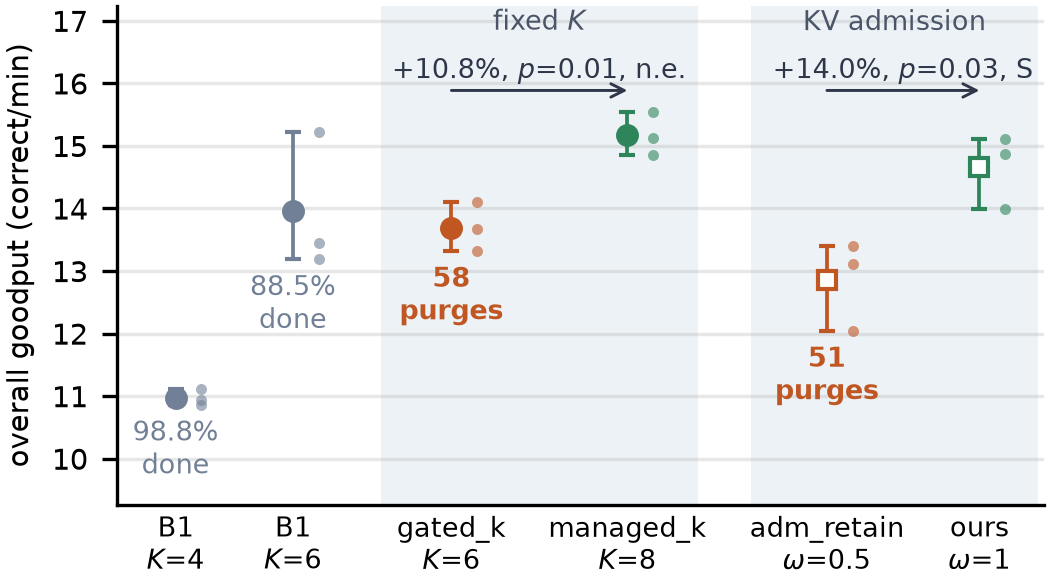
\includegraphics[width=\columnwidth]{../figures/phase2/f2b_dev.png}
  \caption{2\x2 at 16k\,\x4 on dev (mean, min--max, reps). Grey: no gate, orange: llama.cpp
  lifecycle, green: managed; arrows: lifecycle effects (Welch $p$, verdict).}
  \label{fig:decomp}
\end{figure}

\subsection{Decomposition at \texorpdfstring{16k\,\x4}{16k x4}}
Retention under the full gate deadlocks, so \cfg{gated\_k} (fixed \K) and \cfg{adm\_retain} (KV
admission) use an \emph{active gate} (in-flight requests only) and llama.cpp's purge;
\cfg{managed\_k} is fixed \K{} with our lifecycle (Fig.~\ref{fig:decomp}); it uses $K{=}8$, which
ties $K{=}10$ on perf goodput (11.68 vs.\ 11.69) at higher throughput (26.3 vs.\ 25.1): a tie-break
outside the rule, fixed before the dev runs. \emph{Gate (scheduling only):} at
$K{=}6$ the active gate completes all tasks where B1 loses 23 per run, with no significant goodput
change ($-$1.9\%, $p=0.73$\calc). Completing everything lets the 95\% rule choose $K{=}6$ instead of
4, giving +24.8\% over B1\pick{} ($p=0.004$\calc, S): a gain from running a higher \K{} safely, not
from the lifecycle. \emph{Lifecycle:} replacing llama.cpp's purge (58 and 51 purges per run) with
the managed lifecycle (none) adds 14.0\% under KV admission ($p=0.03$, CI [+0.20, +3.89]\calc, S)
and 10.8\% at fixed \K{} ($p=0.01$, but CI [$-$0.58, +3.25]\calc, n.e.). In single tuning runs
(Fig.~\ref{fig:tuning}), \cfg{gated\_k} peaks at $K{=}6$ (11.54) and falls to 7.79 at $K{=}10$ as
purges rise 86$\rightarrow$575; \cfg{managed\_k} holds 11.21--11.69 for $K{=}6$--10. \emph{Admission:} peak projection showed no gain over a tuned fixed \K{} ($-$6.2\%,
$-$3.4\%; n.e.). The pre-registered comparison of ours with the better scheduling-only cell is
+7.0\% ($p=0.09$\calc, n.e.). Most of ours' gain over B1\pick{} is thus already reached by \cfg{gated\_k}
(+24.8\%); which lifecycle components matter is not established.

\subsection{Ablations}\label{sec:abl}
At 16k\,\x4, removing the prefix (\cfg{act\_erase}: $-8.7\%$, one run, 4\x{} the re-prefill) or the
host tier (\cfg{ours\_h0}: $-8.4\%$, $p=0.09$; $-10.2\%$ at 8k\,\x1, $p=0.04$\calc{} but CI includes 0)
gave the largest losses: consistent with both mattering, not established. Single runs changing the
TTL, victim order or delay knowledge stay within $\pm4.3\%$ (ours' reps: 13.98--15.11).
Always offloading instead of the cost-based choice (\cfg{act\_offload}, +4.3\%, 4 reps, $p=0.31$)
and offloading at every tool start (\cfg{always\_off}, +2.4\%, $p=0.44$) are not significantly
different from ours, so the cost model's offload/drop choice is not shown to help. An active-gate bug fixed in tuning
affected only scheduling-only tuning runs (appendix).

\section{Discussion and Limitations}\label{sec:disc}

The full gate kept the pool at its cap with no overflows or purges in 53 runs. At 16k\,\x4 the
managed lifecycle raised goodput over llama.cpp's purge by 11--14\% (one of two effects S);
the TTL, victim ranking and cost-based action choice were not shown to contribute, and
peak-projection admission showed no gain over a tuned fixed \K.
\emph{Limitations.} With 2--4 reps, $p$ is indicative; four comparisons have $p<0.05$ but a CI
including 0. The third rep at 16k\,\x4 and 32k\,\x4 was added because $n=2$ did not separate ours
from B1\pick{} (16k\,\x4: $p=0.09$ at $n=2$), and the \cfg{act\_offload} and \cfg{always\_off} reps
because their single runs looked better, so these $p$-values are optimistic. Deviations from the
spec: overall goodput became the primary test, possibly after dev results were seen
(unrecorded), hence the steady CI in the rule; 8k\,\x1 has 2 reps, not 3; the predicted +5--10\% vs.\
$K{=}4$ at 16k\,\x1 was not met (+1.7\%).
B1's knobs rest on one perf run per \K; the 2\x2 ran only at 16k\,\x4; only dev was run. Ours vs.\ B1 is not iso-memory (up to 448--1,792\,MiB host RAM); \cfg{ours\_h0} is the
iso-memory comparison. B2's low host-cache reuse was not traced. Safety evidence is indirect (no
server cell counts).

\onecolumn
\appendix[Timeline and Milestones]
\vspace{4pt}

\begin{center}
  \small
  \setlength{\tabcolsep}{5pt}
  \begin{tabular}{@{}L{0.11\textwidth}L{0.5\textwidth}L{0.24\textwidth}L{0.08\textwidth}@{}}
    \toprule
    Dates & Work & Milestone & Status \\
    \midrule
    10/21--10/28 & Design; data, corpus, splits; tools, ReAct agent, profiles; workload generator; FIFO
      runner and instrumentation & End-to-end workload on 7B & Done \\
    10/29--10/31 & AWS A10G setup; cost model; runtime probes; microbenchmarks; experiments E1--E5 &
      Measurements and bottleneck analysis & Done \\
    11/1--11/4 & Phase 1 report & \textbf{Phase 1 due 11/4} & Done \\
    11/5--11/15 & Runtime probes for slot controls (E0b, E0c); KV manager: exact ledger and gate,
      peak-projection admission, offload/drop/erase lifecycle with online cost model; cell-level
      llama-server mock; 149 new tests & Manager runs end to end with zero violations (validation
      runs) & Done \\
    11/15--11/16 & Baseline (B1, B2, B3) and $\omega$ tuning on perf; active-gate fix and re-tuning;
      main comparison on dev (2--3 reps, four budget\,\x\,delay points); 2\x2 decomposition;
      ablations; no-benefit regimes & All Phase 2 results & Done \\
    11/16--11/18 & Phase 2 report and technical notes & \textbf{Phase 2 report} & In progress \\
    11/19--11/25 & Close the gaps found in Phase 2: third rep at 8k\,\x1 and 16k\,\x1 (including B1
      $K{=}5$), 2\x2 at 8k\,\x1, confirmation on the 500-task test split & Phase 2 claims tested on
      held-out data (test split) & Planned \\
    11/23--11/30 & Remaining pre-registered sweeps: delay scale, default mix, Poisson arrivals
      (latency), iso-GPU-memory comparison & Robustness of the gain & Planned \\
    11/26--12/2 & Phase 3 (optional): selective KV, trimming non-evidence observation text at tool
      boundaries with HotpotQA supporting facts as oracle (text-level compaction first) & Quality vs.\
      KV trade-off & Optional \\
    12/3--12/9 & Final report and reproducibility package & \textbf{Final submission 12/9} & Planned \\
    \bottomrule
  \end{tabular}
\end{center}

\begin{figure}[h]
  \centering
  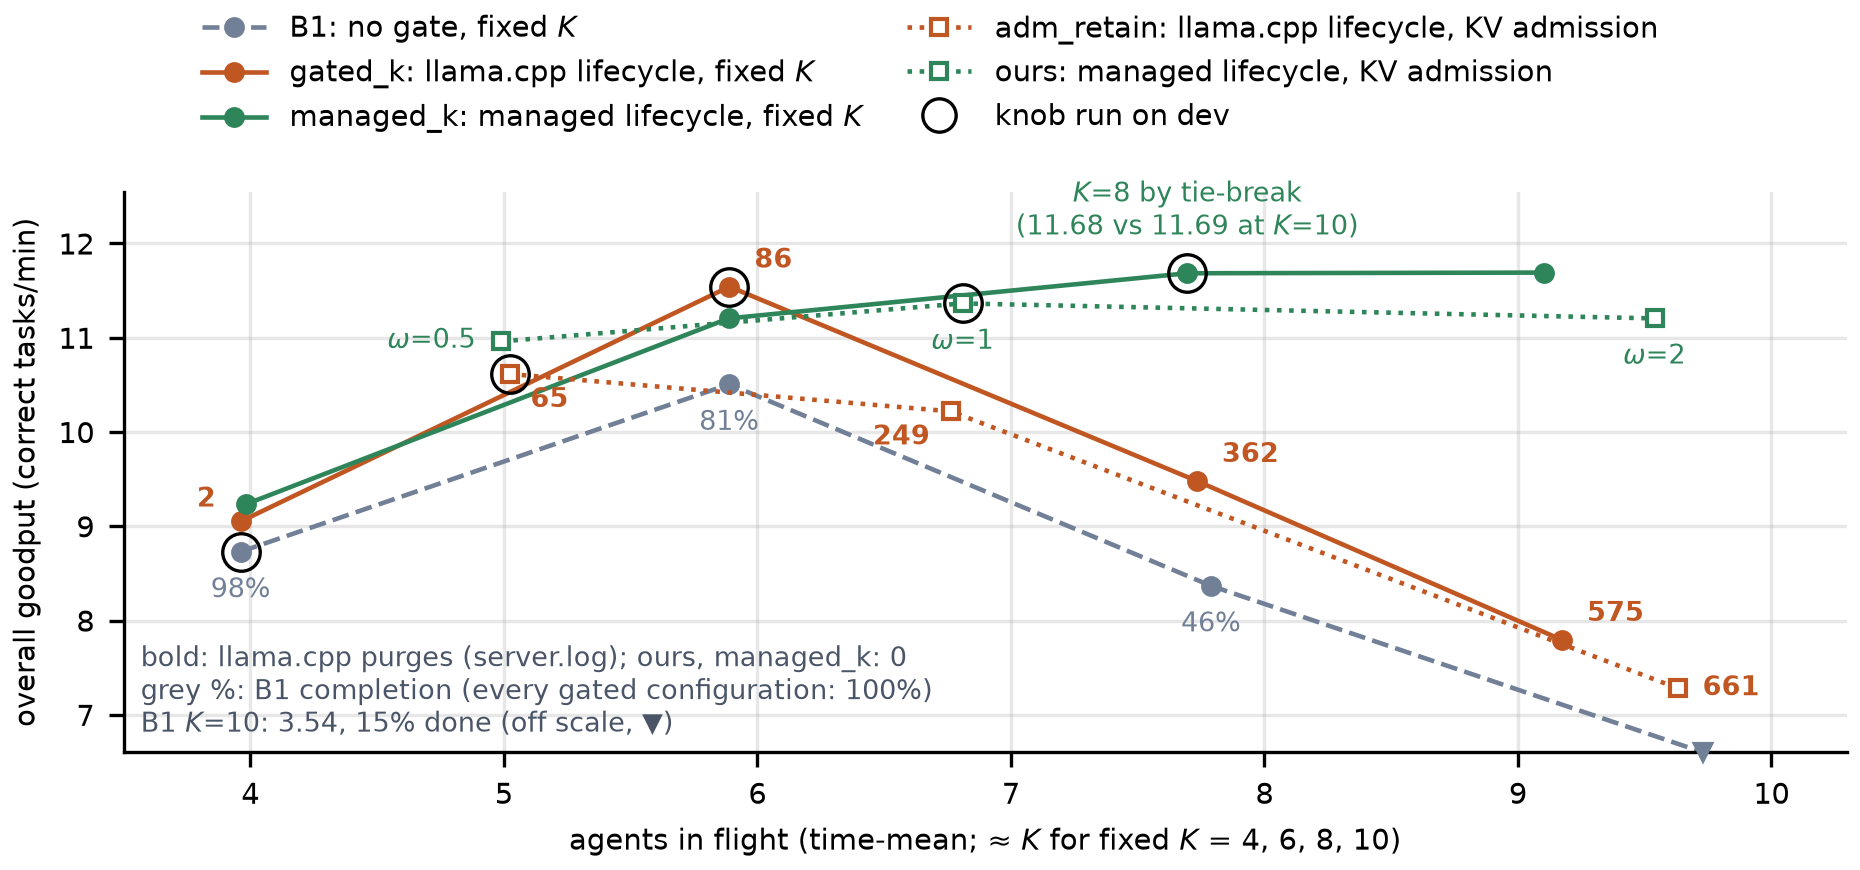
\includegraphics[width=6.2in]{../figures/phase2/f2a_tuning.png}
  \caption{Perf tuning runs at 16k\,\x4, one per knob (selection data, not results). Circles = knob
  run on dev in Fig.~\ref{fig:decomp} (\cfg{managed\_k}: $K{=}8$ by tie-break; the goodput rule gives
  $K{=}10$); bold = llama.cpp purges per run; grey \% = B1 completion.}
  \label{fig:tuning}
\end{figure}

\noindent\emph{Active-gate bug.} In tuning, two of three \cfg{adm\_retain} runs overflowed: the
active gate charged a reused slot at $f$ instead of $\max(s,f)$ (from the source, llama.cpp drops
the old tail only when the prompt enters a batch). All three pre-fix \cfg{adm\_retain} runs were
excluded and the cell re-tuned. Only the two scheduling-only cells use this gate; the full-gate
configurations and all dev runs are unaffected (the revision is inferred from end-of-run hashes).

\begin{thebibliography}{4}
\footnotesize
\bibitem{llamacpp} G.~Gerganov \emph{et al.}, ``llama.cpp,'' \url{https://github.com/ggml-org/llama.cpp}.
\bibitem{qwen} Qwen Team, ``Qwen2.5 technical report,'' arXiv:2412.15115, 2024.
\bibitem{hotpotqa} Z.~Yang \emph{et al.}, ``HotpotQA: A dataset for diverse, explainable multi-hop question
answering,'' in \emph{Proc. EMNLP}, 2018.
\bibitem{react} S.~Yao \emph{et al.}, ``ReAct: Synergizing reasoning and acting in language models,'' in
\emph{Proc. ICLR}, 2023.
\end{thebibliography}

\end{document}
